% (C) Copyright 2016
% Urs Fässler, www.bitzgi.ch
% SPDX-License-Identifier: CC-BY-SA-4.0

\subsection{Grundlagen}
\label{sec:voraussetzungen}
\subsectionframe

\begin{frame}
	\begin{center}
		\begin{tikzpicture}
		[
			node distance = 3 cm,
			box/.style = {thick, draw=black, top color=white, bottom color=lightblue, rounded corners, align=center, inner sep = 0.5cm},
			can/.style={->, very thick, shorten <=0.2cm, shorten >=0.2cm,}
		]
		
		\visible<1-> {
			\node[box] (freedom) {Freie Software};
		}
		
		\visible<2-> {
			\node[box, above right of = freedom] (run) {Verwenden\only<handout>{\\Die Freiheit, die Software uneingeschränkt und für jeden Zweck einzusetzen.}};
			\draw[can] (freedom) -> (run);
		}
	
		\visible<3-> {
			\node[box, above left of = freedom] (study) {Verstehen\only<handout>{\\Die Freiheit, die Funktionsweise der Software untersuchen und verstehen zu können.}};
			\draw[can]  (freedom) -> (study);
		}
	
		\visible<4-> {
			\node[box, below left of = freedom] (redistribute) {Verbreiten\only<handout>{\\Die Freiheit, Kopien der Software zu verbreiten, um damit seinen Mitmenschen zu helfen.}};
			\draw[can]  (freedom) -> (redistribute);
		}
	
		\visible<5-> {
			\node[box, below right of = freedom] (improve) {Verbessern\only<handout>{\\Die Freiheit, die Software zu verbessern und die Verbesserungen an die Öffentlichkeit weiterzugeben, sodass die gesamte Gesellschaft davon profitieren kann.}};
			\draw[can]  (freedom) -> (improve);
		}
	
		\end{tikzpicture}
	\end{center}
\end{frame}
\note
{
	\url{http://www.inf-schule.de/software/freie\_software/02\_freiheiten\_freier\_software}
}

\begin{frame}{Frei und Kommerziell}
	\begin{center}
		\begin{tabular}{c|c|c|}
			 & \visible<3->{\thead{proprietär}} & \visible<2->{\thead{frei}} \\ 
			\hline 
			\visible<4->{\thead{gratis}} & \visible<6->{\makecell{(iOS)\\Freeware}} & \visible<7->{\makecell{Debian\\GNU/Linux}}\\ 
			\hline 
			\visible<4->{\thead{kommerziell}} & \visible<5->{\makecell{Windows\\Mac OS}} & \visible<8->{\makecell{Red Hat Enterprise\\Linux}}\\ 
			\hline 
		\end{tabular} 
	\end{center}
\end{frame}

\begin{frame}{Intellectual Property (IP)}
	\begin{center}
		\visible<2->{\large Geistiges Eigentum}
		\begin{tabular}{ccc}
		\hspace{3cm} & \hspace{3cm} & \hspace{3cm} \\
		\visible<3->{Patent} & \visible<4->{Markenrecht} & \visible<5->{Urheberrecht} \\ 
		\visible<3->{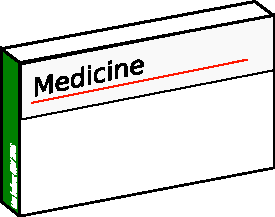
\includegraphics[height=2cm]{res/tulipan-Pharmaceutical-carton.pdf}} & \visible<4->{
\includegraphics[height=2.5cm]{res/gnu-head.pdf}} & \visible<5->{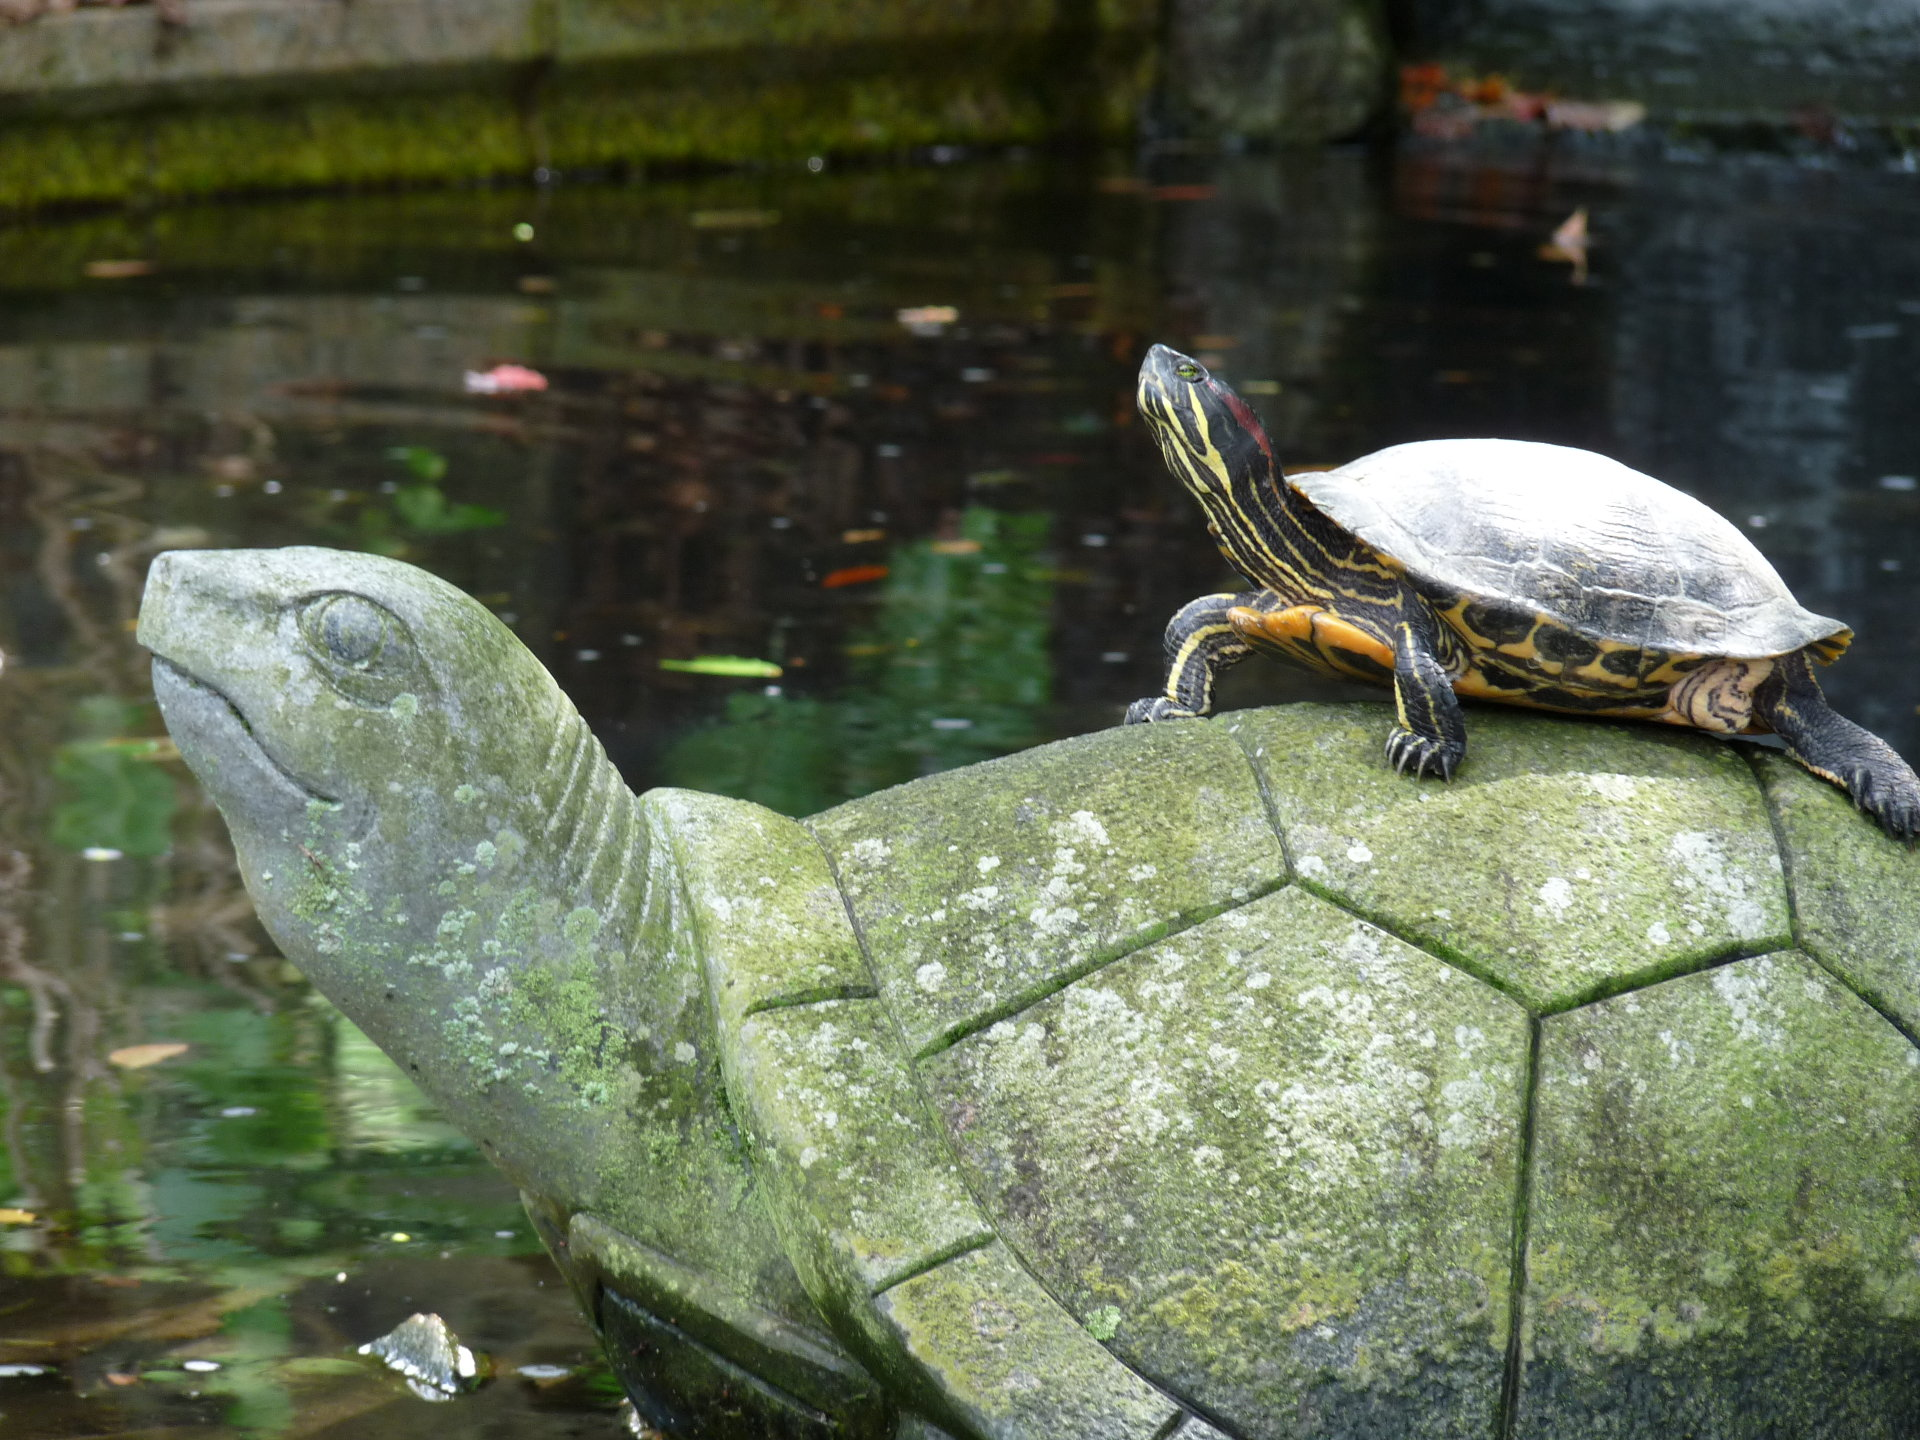
\includegraphics[height=2.5cm]{res/turtles.jpg}} \\ 
		\only<handout>
		{
			Auf Antrag & Auf Antrag & automatisch \\
			\makecell{Schutz der\\Investition} & \makecell{Schutz von\\Erkennungsmerkmal} & \makecell{Verwertungsrecht\\künstlerischer\\Schöpfungen} \\
			20 Jahre & beliebig erneuerbar & 70 Jahre nach Tod \\
		}
		\end{tabular} 
	\end{center}
\end{frame}
\note
{
	(IP, Intellectual Property, Geistiges Eigentum) \url{https://de.wikipedia.org/wiki/Geistiges\_Eigentum\#Systematik}
	\begin{itemize}
		\item Patent
		\item Markenrecht
		\item Urheberrecht
	\end{itemize}
}
\note
{
	\begin{itemize}
		\item Patent
		\begin{itemize}
			\item \url{https://de.wikipedia.org/wiki/Patent}
			\item Defensivpublikation
			\item Acarton with pills: CC-0 by tulipan \url{https://openclipart.org/detail/6135/pharmaceutical-carton}
		\end{itemize}
	\end{itemize}
}
\note
{
	\begin{itemize}
		\item Markenrecht
		\begin{itemize}
			\item \url{https://de.wikipedia.org/wiki/Marke_(Recht)}
			\item Firefox und Debian (Iceweasel): \url{https://lwn.net/Articles/676799/}
			\item A GNU Head: CC-BY-SA Etienne Suvasa; Trademark of the GNU Project: \url{https://www.gnu.org/graphics/agnuhead.html}
		\end{itemize}
	\end{itemize}
}
\note
{
	\begin{itemize}
		\item Urheberrecht
		\begin{itemize}
			\item \url{https://de.wikipedia.org/wiki/Urheberrecht}
			\item für Werke
			\item daher auch für Software
			\item gilt automatisch: \url{https://anwalt-im-netz.de/urheberrecht/urheberrecht-faq.html\#wann}
			\item Copyrightzeichen ist nicht nötig: \url{https://de.wikipedia.org/wiki/Copyrightzeichen}
			\item Nicht verzichtbar (kein public domain, Gemeinfreiheit: \url{https://de.wikipedia.org/wiki/Gemeinfreiheit\#Entlassung\_in\_die\_Gemeinfreiheit})
		\end{itemize}
	\end{itemize}
}
